% Options for packages loaded elsewhere
\PassOptionsToPackage{unicode}{hyperref}
\PassOptionsToPackage{hyphens}{url}
\PassOptionsToPackage{dvipsnames,svgnames,x11names}{xcolor}
%
\documentclass[
  letterpaper,
  DIV=11,
  numbers=noendperiod]{scrartcl}

\usepackage{amsmath,amssymb}
\usepackage{iftex}
\ifPDFTeX
  \usepackage[T1]{fontenc}
  \usepackage[utf8]{inputenc}
  \usepackage{textcomp} % provide euro and other symbols
\else % if luatex or xetex
  \usepackage{unicode-math}
  \defaultfontfeatures{Scale=MatchLowercase}
  \defaultfontfeatures[\rmfamily]{Ligatures=TeX,Scale=1}
\fi
\usepackage{lmodern}
\ifPDFTeX\else  
    % xetex/luatex font selection
\fi
% Use upquote if available, for straight quotes in verbatim environments
\IfFileExists{upquote.sty}{\usepackage{upquote}}{}
\IfFileExists{microtype.sty}{% use microtype if available
  \usepackage[]{microtype}
  \UseMicrotypeSet[protrusion]{basicmath} % disable protrusion for tt fonts
}{}
\makeatletter
\@ifundefined{KOMAClassName}{% if non-KOMA class
  \IfFileExists{parskip.sty}{%
    \usepackage{parskip}
  }{% else
    \setlength{\parindent}{0pt}
    \setlength{\parskip}{6pt plus 2pt minus 1pt}}
}{% if KOMA class
  \KOMAoptions{parskip=half}}
\makeatother
\usepackage{xcolor}
\setlength{\emergencystretch}{3em} % prevent overfull lines
\setcounter{secnumdepth}{-\maxdimen} % remove section numbering
% Make \paragraph and \subparagraph free-standing
\makeatletter
\ifx\paragraph\undefined\else
  \let\oldparagraph\paragraph
  \renewcommand{\paragraph}{
    \@ifstar
      \xxxParagraphStar
      \xxxParagraphNoStar
  }
  \newcommand{\xxxParagraphStar}[1]{\oldparagraph*{#1}\mbox{}}
  \newcommand{\xxxParagraphNoStar}[1]{\oldparagraph{#1}\mbox{}}
\fi
\ifx\subparagraph\undefined\else
  \let\oldsubparagraph\subparagraph
  \renewcommand{\subparagraph}{
    \@ifstar
      \xxxSubParagraphStar
      \xxxSubParagraphNoStar
  }
  \newcommand{\xxxSubParagraphStar}[1]{\oldsubparagraph*{#1}\mbox{}}
  \newcommand{\xxxSubParagraphNoStar}[1]{\oldsubparagraph{#1}\mbox{}}
\fi
\makeatother


\providecommand{\tightlist}{%
  \setlength{\itemsep}{0pt}\setlength{\parskip}{0pt}}\usepackage{longtable,booktabs,array}
\usepackage{calc} % for calculating minipage widths
% Correct order of tables after \paragraph or \subparagraph
\usepackage{etoolbox}
\makeatletter
\patchcmd\longtable{\par}{\if@noskipsec\mbox{}\fi\par}{}{}
\makeatother
% Allow footnotes in longtable head/foot
\IfFileExists{footnotehyper.sty}{\usepackage{footnotehyper}}{\usepackage{footnote}}
\makesavenoteenv{longtable}
\usepackage{graphicx}
\makeatletter
\newsavebox\pandoc@box
\newcommand*\pandocbounded[1]{% scales image to fit in text height/width
  \sbox\pandoc@box{#1}%
  \Gscale@div\@tempa{\textheight}{\dimexpr\ht\pandoc@box+\dp\pandoc@box\relax}%
  \Gscale@div\@tempb{\linewidth}{\wd\pandoc@box}%
  \ifdim\@tempb\p@<\@tempa\p@\let\@tempa\@tempb\fi% select the smaller of both
  \ifdim\@tempa\p@<\p@\scalebox{\@tempa}{\usebox\pandoc@box}%
  \else\usebox{\pandoc@box}%
  \fi%
}
% Set default figure placement to htbp
\def\fps@figure{htbp}
\makeatother
% definitions for citeproc citations
\NewDocumentCommand\citeproctext{}{}
\NewDocumentCommand\citeproc{mm}{%
  \begingroup\def\citeproctext{#2}\cite{#1}\endgroup}
\makeatletter
 % allow citations to break across lines
 \let\@cite@ofmt\@firstofone
 % avoid brackets around text for \cite:
 \def\@biblabel#1{}
 \def\@cite#1#2{{#1\if@tempswa , #2\fi}}
\makeatother
\newlength{\cslhangindent}
\setlength{\cslhangindent}{1.5em}
\newlength{\csllabelwidth}
\setlength{\csllabelwidth}{3em}
\newenvironment{CSLReferences}[2] % #1 hanging-indent, #2 entry-spacing
 {\begin{list}{}{%
  \setlength{\itemindent}{0pt}
  \setlength{\leftmargin}{0pt}
  \setlength{\parsep}{0pt}
  % turn on hanging indent if param 1 is 1
  \ifodd #1
   \setlength{\leftmargin}{\cslhangindent}
   \setlength{\itemindent}{-1\cslhangindent}
  \fi
  % set entry spacing
  \setlength{\itemsep}{#2\baselineskip}}}
 {\end{list}}
\usepackage{calc}
\newcommand{\CSLBlock}[1]{\hfill\break\parbox[t]{\linewidth}{\strut\ignorespaces#1\strut}}
\newcommand{\CSLLeftMargin}[1]{\parbox[t]{\csllabelwidth}{\strut#1\strut}}
\newcommand{\CSLRightInline}[1]{\parbox[t]{\linewidth - \csllabelwidth}{\strut#1\strut}}
\newcommand{\CSLIndent}[1]{\hspace{\cslhangindent}#1}

\KOMAoption{captions}{tableheading}
\makeatletter
\@ifpackageloaded{caption}{}{\usepackage{caption}}
\AtBeginDocument{%
\ifdefined\contentsname
  \renewcommand*\contentsname{Table of contents}
\else
  \newcommand\contentsname{Table of contents}
\fi
\ifdefined\listfigurename
  \renewcommand*\listfigurename{List of Figures}
\else
  \newcommand\listfigurename{List of Figures}
\fi
\ifdefined\listtablename
  \renewcommand*\listtablename{List of Tables}
\else
  \newcommand\listtablename{List of Tables}
\fi
\ifdefined\figurename
  \renewcommand*\figurename{Figure}
\else
  \newcommand\figurename{Figure}
\fi
\ifdefined\tablename
  \renewcommand*\tablename{Table}
\else
  \newcommand\tablename{Table}
\fi
}
\@ifpackageloaded{float}{}{\usepackage{float}}
\floatstyle{ruled}
\@ifundefined{c@chapter}{\newfloat{codelisting}{h}{lop}}{\newfloat{codelisting}{h}{lop}[chapter]}
\floatname{codelisting}{Listing}
\newcommand*\listoflistings{\listof{codelisting}{List of Listings}}
\makeatother
\makeatletter
\makeatother
\makeatletter
\@ifpackageloaded{caption}{}{\usepackage{caption}}
\@ifpackageloaded{subcaption}{}{\usepackage{subcaption}}
\makeatother

\usepackage{bookmark}

\IfFileExists{xurl.sty}{\usepackage{xurl}}{} % add URL line breaks if available
\urlstyle{same} % disable monospaced font for URLs
\hypersetup{
  pdftitle={The trials of interpreting clinical trials - A Bayesian perspective},
  colorlinks=true,
  linkcolor={blue},
  filecolor={Maroon},
  citecolor={Blue},
  urlcolor={Blue},
  pdfcreator={LaTeX via pandoc}}


\title{The trials of interpreting clinical trials - A Bayesian
perspective}
\author{James M Brophy}
\date{}

\begin{document}
\maketitle
\begin{abstract}
Importance: Evidence based medicine (EBM) paradigm places systematic
reviews and meta-analyses, ideally of randomized clinical trials (RCTs),
at the top of the evidential pyramid. However, resolving situations with
``conflicting'' or ``missing'' evidence can be problematic:\\
Observations: This is a case-based review of Bayesian techniques to
assist in optimizing the interpretation of well performed RCTs with
conflicting evidence. Using the example of cochicine in post acute
myocardial infarction subjects, it is demonstrated how these techniques
avoid common interpretative cognitive biases, provide additional
analytical nuances, and thereby enhancing the original published
conclusions.\\
Conclusions and Relevance: If the trials are of equal high quality,
conflicts are often illusory arising from the improper comparisons of
statistical significance. Current statistical approaches which ignore
prior evidence and rely on null hypothesis significance testing lead to
vacillating beliefs that do not always faithfully respect the laws of
probability and consequently may not align with the true state of
knowledge. Bayesian techniques can address these issues and raisr the
quality of clinical trial interpretations.
\end{abstract}


\subsection{Introduction}\label{introduction}

Evidence based medicine (EBM) paradigm places systematic reviews and
meta-analyses, ideally of randomized clinical trials, at the top of the
evidential pyramid. A less studied, but recurring question is how to
approach decision making with ``conflicting'' or ``missing'' evidence.
While this commentary will explore various statistical answers, it must
be appreciated that these are only ancillary methods to the crucial
element of clinical judgement. In an analogous manner to statistical
significance not equating to causality, clinical judgement must precede
statistical analyses in deciding what is in fact ``combinable''.

\subsection{A recent example}\label{a-recent-example}

In the CLEAR OASIS 9 trial(1), acute myocardial infarction (AMI)
patients were randomized to colchicine (n = 3,528) or placebo (n =
3,534) immediately after percutaneous coronary intervention (PCI). The
primary outcome was major adverse cardiovascular events (MACE), a
composite of cardiovascular (CV) death, MI, stroke, or ischemia-driven
revascularization. With a median 3 year follow-up, there were 9.1\%
events in the colchicine group and 9.3\% in the placebo arm, hazard
ratio (HR) 0.99 (95\% confidence interval {[}CI{]} 0.85-1.16, p = 0.93).
Given the high quality of the study design and its execution as well as
the large number of primary-outcome events (649), the authors reasoned
that the chance of a spurious result was low. Thus, they concluded
``\ldots{} treatment with colchicine, when started soon after myocardial
infarction and continued for a median of 3 years, did not reduce the
incidence of the composite primary outcome.''\\
CLEAR authors acknowledge that the most comparable previous study was
COLCOT(2), a randomized trial of 4745 patients who received the same 0.5
mg daily colchicine dose (n=2366) or placebo within 30 days of an AMI
and were followed for a median of 22.6 months. Their primary outcome was
a composite (cardiovascular deaths, recurrent myocardial infarction,
resuscitation after cardiac arrest, stroke, or urgent hospitalization
for angina that led to revascularization), very similar to the CLEAR
outcome. This trial had a total of 301 primary-outcome events, and
colchicine treatment was associated with a 23\% relative reduction
(hazard ratio, 0.77; 95\% {[}CI{]}, 0.61 to 0.96; P = 0.02). In the
CLEAR discussion(1), there was no attempt to explain these
``differences'' other than observing that two other recent colchicine
trials in stroke patients{[}(3){]}(4) also showed no benefit with
colchicine and that CLEAR was a bigger trial, presumably with an
improved precision of the treatment effect.\\
What now should the average clinician now believe? Should they adopt the
implicit CLEAR investigators' view that since that trial is larger it
should be believed and that the evidence from the 4745 COLCOT patients
should simply be forgotten or ignored. The CLEAR PI was more explicit in
an interview following the oral presentation of their findings stating
that before CLEAR ``I was a believer in colchicine,'' (implictly because
of COLCOT(?), although this belief presumably wasn't universally shared
or the necessary equipoise would not have been present to proceed with
the CLEAR trial) but after CLEAR ``I decided to stop it in my
parent''(5). This dichotomization of beliefs is common among clinicians,
undoubtedly influenced by the null hypothesis significance testing
paradigm and the conventional p value 0.05 threshold used in medical
research. This approach encourages deterministic binary viewpoints not
only for accepting or rejecting null hypotheses but also for clinical
decision making.\\
On the other hand, some may may prefer to wait for a meta-analysis
incorporating all available colchicine studies before formulating their
opinion. Of course, care must be taken to assure the consistency of
study design, patient populations, and outcomes of any included studies.
But what if there are no meta-analyses or even more disconcerting, no
comparable previous trials at all? Is there another approach that
facilitates a more nuanced interpretation of randomized trials like
CLEAR either with, or without, the existence of prior knowledge?\\

\subsection{The Bayesian approach}\label{the-bayesian-approach}

As mentioned above, the common statistical paradigm in medical research
is null hypothesis significance testing (NHST) where decisions are
conditioned on the comparison of p values (P (observed or more extreme
data \textbar{} a statistical model and null hypothesis)\footnote{Shorthand
  for ``Probability (observed or more extreme data given a statistical
  model and null hypothesis)''} to prespecified type I errors.
Unfortunately this approach may result in cognitive
errors{[}(6){]}(7)(8). On the other hand, a Bayesian approach provides
the information clinicians are actually seeking, namely the probability
that the hypothesis is true given the observed data, P (hypothesis
\textbar{} observed data). This posterior distribution, derived from a
weighted combination of a prior belief and the current data, not only
allows the incorporation of prior knowledge according to the rules of
probability, when available, but also avoids the aforementioned
cognitive errors.

\subsubsection{Vague priors}\label{vague-priors}

Bayesian analyses can use differing prior beliefs thereby providing an
assessment of the overall robustness of the posterior conclusions.
Adopting the CLEAR viewpoint of trial interpretation independently of
any prior knowledge, a vague prior would be chosen for the Bayesian
analysis so that the posterior probability distribution is completely
dominated by the observed CLEAR data. An advantage of probability
distributions is they are not restricted to specific point estimates but
permit calculations for multiple different cutpoints or intervals. For
example, one might be particularly interested in probabilities exceeding
a clinically meaningful thresholds for benefit or harm. Such clinical
cutpoints can be individually selected but for demonstration purposes, a
benefit threshold of RR \textless{} 0.9 and harm threshold of RR
\textgreater{} 1.1 as been chosen.

For CLEAR data with vague priors, the probabilities of clinical benefit
(RR \textless{} 0.9), practical equivalence ( 0.9 \textless{} RR
\textless{} 1.1) and harm (RR \textgreater{} 1.1) are 12.375\%, 81.2\%
and 6.425\%, respectively. The probability of any benefit (RR
\textless{} 1) is 60.45\%. These results are shown graphically in Figure
1, where the area under the curve is proportional to each probability.
This analysis thus shows a small, but not trivial residual probability
(12.4\%) for a clinically significant benefit (as arbitrarily defined by
a minimum 10\% decrease in RR).~

Some clinicians might interpret these results not as a rejection of the
colchicine hypothesis as proposed by the CLEAR investigators but rather
alternatively as showing that while somewhat unlikely the possibility of
a colchicine benefit remains and that additional studies or analyses are
required to refine these estimates. However if a clinician was a priori
a colchicine ``believer'' this vague prior of this analysis should be
replaced by the appropriate informative prior. Informative priors, like
vague priors, are be combined with the current data according to Bayes
Theorem and follow the laws of probability, i.e.~a weighted average with
weights proportional to the precision of the prior and current data.

\subsubsection{Informative priors}\label{informative-priors}

Given that CLEAR(1) and COLCOT(2) were both well designed, well executed
trials examining the same intervention in the same study populations and
published in the same esteemed medical journal, its seems absurd to
ignore either of them. A fundamental question is are these two study
results really different? From a statistical perspective the trials
aren't radically different with overlapping 95\% CIs. It is only if each
trial is assessed with the dichotomous statistical significance lens
that the two trials appear different. There are no substantive reason
explaining this ersatz statistical heterogeneity given the same
interventions in similar populations with the same measured outcome. The
key insight being ``In making a comparison between two treatments, one
should look at the statistical significance of the difference rather
than the difference between their significance levels(9). The Bayesian
statistical lens will sharpen this perspective.\\

First, COLCOT results can be analyzed within a Bayesian framework, again
with a vague prior so results are dependent uniquely on the COLCOT data.
The probabilities of clinical benefit (RR \textless{} 0.9), practical
equivalence ( 0.9 \textless{} RR \textless{} 1.1) and harm (RR
\textgreater{} 1.1) are 89.975\%, 9.85\% and 0.175\%, respectively. The
probability of a clinical benefit exceeding a 20\% reduction is 59.85\%
and the probability of any benefit, 98.65\% (see Figure 2).

This figure explains why before CLEAR, some clinicians were ``colchicine
believers'' and other were not. Some will be enthusiastic about a 90\%
probability of a clinical benefit (assuming a 10\% reduction in RR is an
appropriate clinical threshold). Those willing to accept this benefit
threshold might classify themselves initially as ``colchicine
believers''. Others may be more conservative and want a larger reduction
in RR, given the inconvenience, cost, and possible side effects of
adding another medication. The probability of an at least 20\% reduction
in RR was only 60\%, not much better than a coin toss, underscoring a
willingness to wait for, and even participate in, further studies
(CLEAR) to better define clinical benefits.\\

Accepting the validity of both trials, what should one now believe after
CLEAR, if the prior belief is well represented by COLCOT data. The only
change to the previous Bayesian analysis is to replace the vague prior
with this informative prior. The results are displayed graphically in
Figure 3 where the posterior distribution is now a weighted average
between the COLCOT probability distribution (prior) and the CLEAR
likelihood distribution.\\
Consider the colchicine ``believer'' prior to CLEAR but not afterwards.
If COLCOT was responsible for the initial positive prior belief, this
analyse suggests after CLEAR there remains a 40.9\% probability of a
clinically meaningful decrease in CV risk with colchicine, a 58.975\%
probability of clinical equivalence with placebo and virtually no chance
of a clinically meaningful increase in harm. Of course, if a clinician
had an clinical cutpoint for efficacy of RR \textless{} 0.80 then it
does indeed seem reasonable, based on the totality of the evidence to be
a ``non-believer'' after CLEAR as the probability of a decrease in
cardiovascular outcomes of this magnitude is less than 1.775\%. However
consistency would imply that their prior belief should also be
referenced to a probability of RR \textless{} 0.80 which for COLCOT was
only 60\%. This seems a fairly modest probability to have been a
``believer'' in this therapy before the current study.\\
This example demonstrates that an intuitive reconciliation of prior and
posterior beliefs can be difficult and is not facilitated by
dichotomized reasoning. Moreover, clinicians may exhibit an availability
bias whereby they are overly influenced by the last trial, particularly
if they were intimately involved in it. The probabilistically correct
harmonization of all available evidence with a Bayesian analysis can
mininmize these cognitive errors.\\

\subsubsection{Bayesian Meta-analysis}\label{bayesian-meta-analysis}

Updating prior beliefs is temporally consistent with data availability
and mirrors human sequential learning. Similar results are nevertheless
reached with Bayesian random effects (hierarchical) meta-analysis when
data temporality is not considered. Individual studies are then treated
as part of a larger population of studies and allows for ``shrinkage'',
where individual study estimates are partially ``pulled'' toward the
overall mean effect. Hierarchical models represent a compromise between
complete pooling (fixed effect) or no pooling (study independency).\\
Hierarchical models accounts for both within and between study
variability producing pooled mean estimates that integrate information
from different studies while acknowledging that individual study effects
might vary. These models also can provide the predictive interval for
the next study from the super population of possible studies. Again in
the Bayesian paradigm, all parameters require an initial priors and a
meta-analysis of the colchicine studies using vague priors is displayed
in Figure 4.

The figure demonstrates several key points;\\
1. there is shrinkage of each observed trial result towards the global
mean\\
2. the global mean is a normal(0.896, 0.386) distribution and
P(colchicine benefit \textgreater{} 10\% RR reduction) = 50\%\\
3. the probability result approaches that obtained from the previous
sequential Bayesian approach

\subsubsection{Bayesian meta-analysis with a single
trial}\label{bayesian-meta-analysis-with-a-single-trial}

While hierarchical meta-analyses account for both within study and
between study variability, a procedural question arises if there is only
one study. In this case, a paradoxical situation arises due to between
study variation being unmeasurable. Consequently the single study
without this between study variation estimate appears to provide better
precision in estimating the mean population effect than when more
evidence is avaialble in the form of multiple studies with thier between
study heterogeneity which is typically not equal to zero.\\
Compared to naively ignoring this between study variation, a recent
study of single studies (10) showed an empirical Bayes approach using as
a prior the distribution of treatment effects and heterogeneity from the
1,636 meta-analyses in the Cochrane Database of Systematic Reviews
showed reductions in the mean squared error for estimating the
study-level and population-level effects.\\
For the CLEAR example, this novel approach gives a 58\% probability of a
positive effect and a 10\% probability that the effect exceeds a 10\% RR
reduction, a consistent answer with the previous analysis with vague
priors.

\subsection{Conclusion}\label{conclusion}

Clinicians are often faced with ``conflicting'' trial evidence. However
if the trials are of equal high quality, often these conflicts are
illusory arising from the improper comparisons of statistical
significance. Systematic reviews and meta-analyses of prior evidence are
now de riguer before a study is considered for peer review funding. Yet
there is no similar mandate for evidence synthesis upon trial
completion. Indeed current incentives strongly favor each trial being
individually interpreted. However, as demonstrated in the colchicine
trials, this approach can lead to vacillating beliefs that do not
respect the laws of probability and consequently may not align with the
true state of knowledge. Bayesian techniques can address these issues
thereby raising the quality of clinical trial interpretations.\\

\subsection{Figures}\label{figures}

\pandocbounded{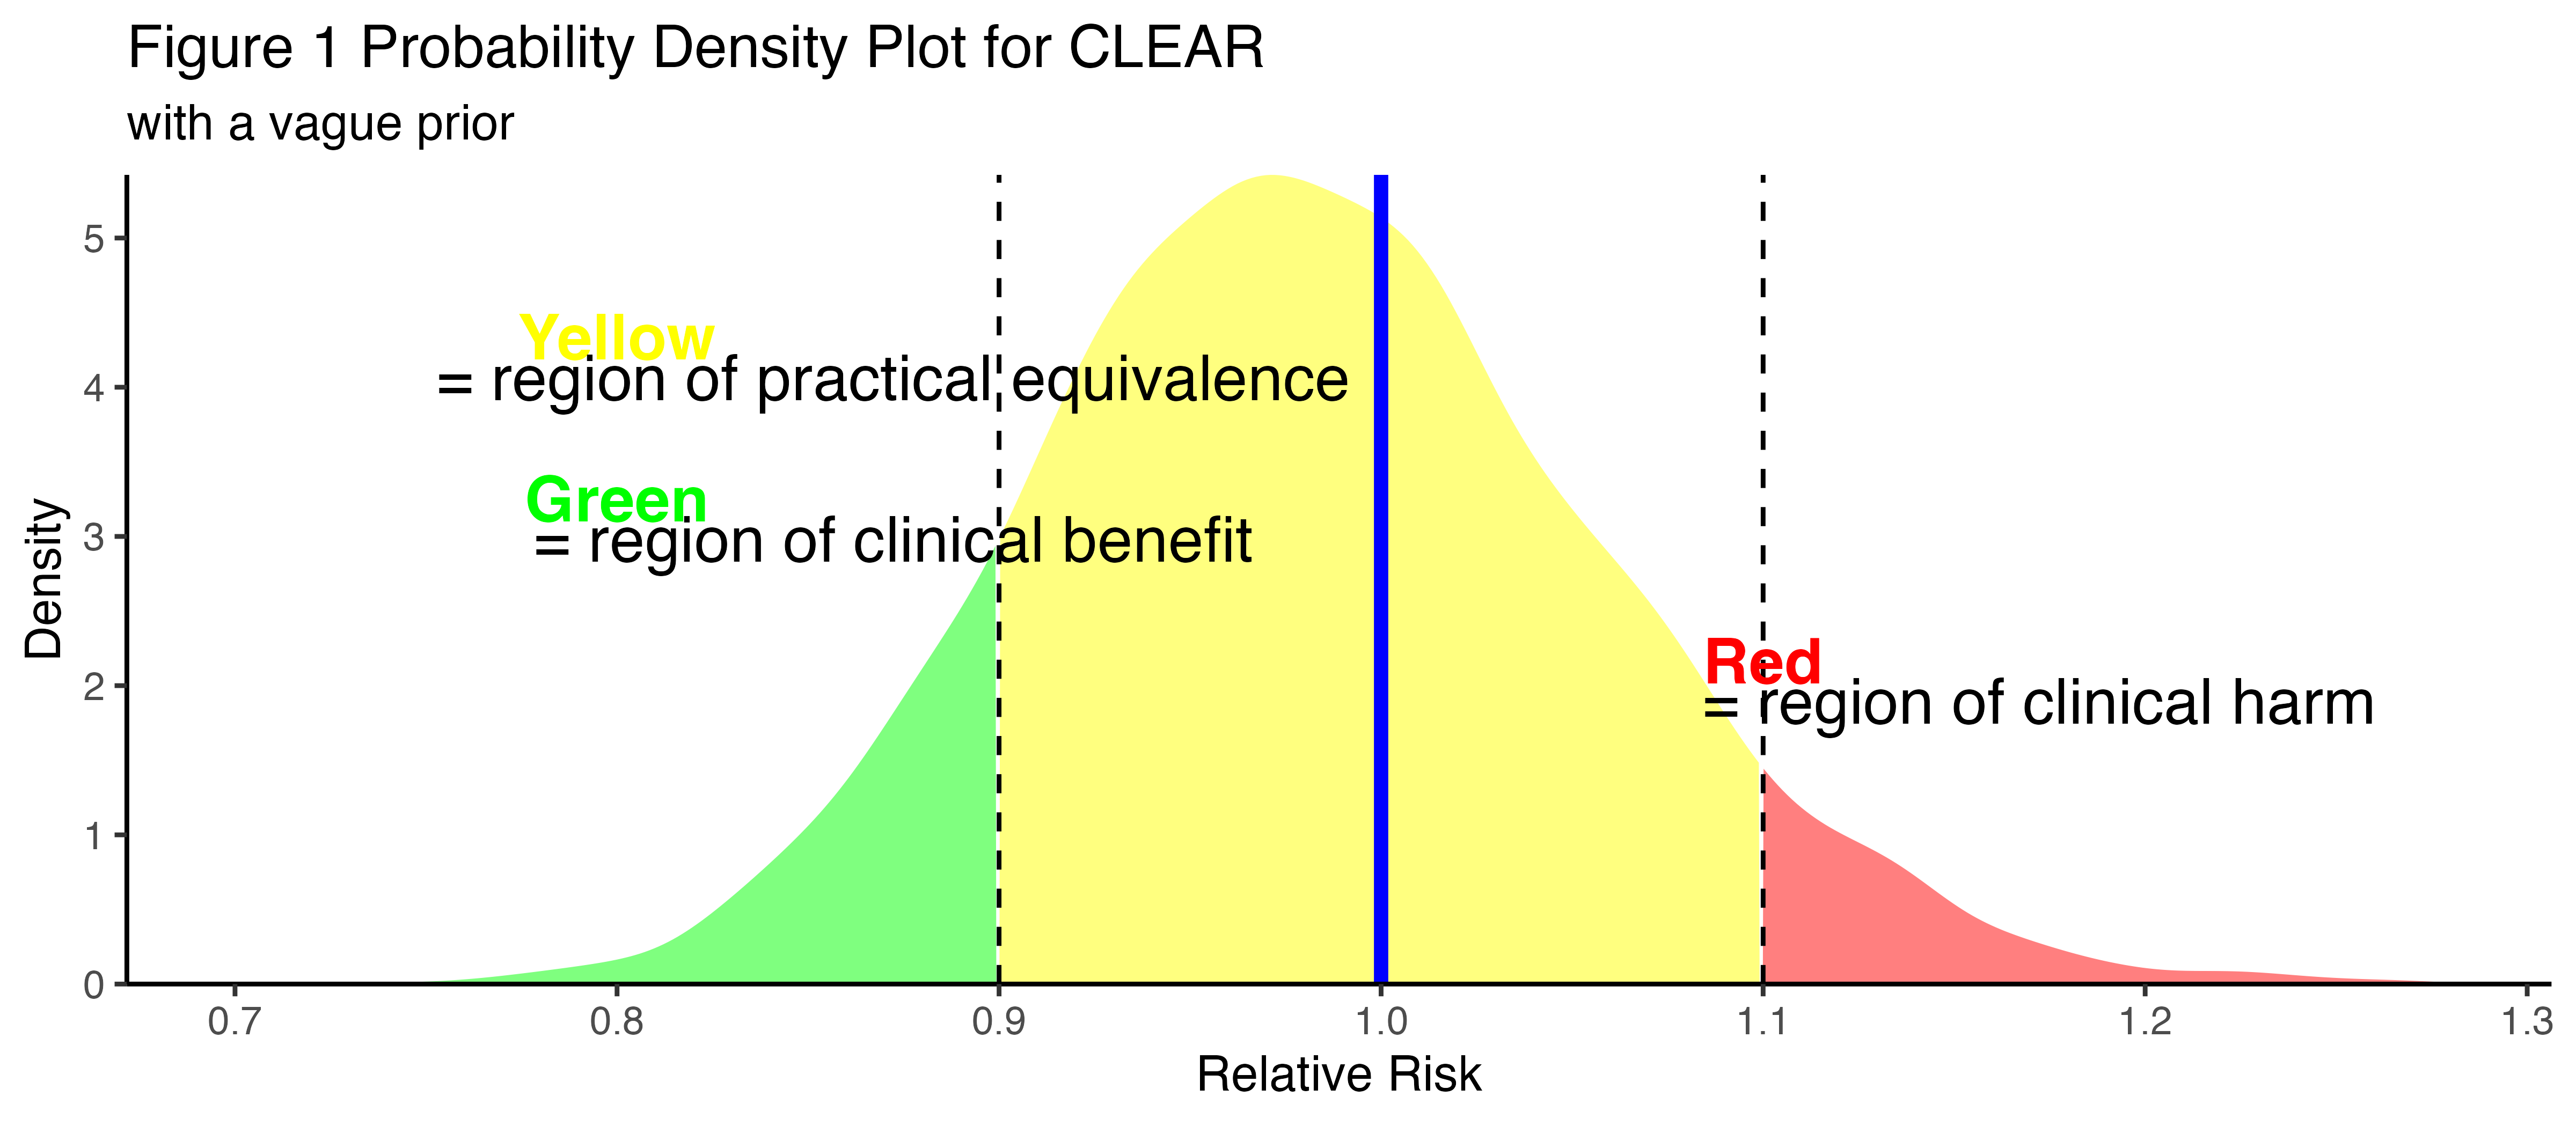
\includegraphics[keepaspectratio]{output/clear_vague.png}}~
\pandocbounded{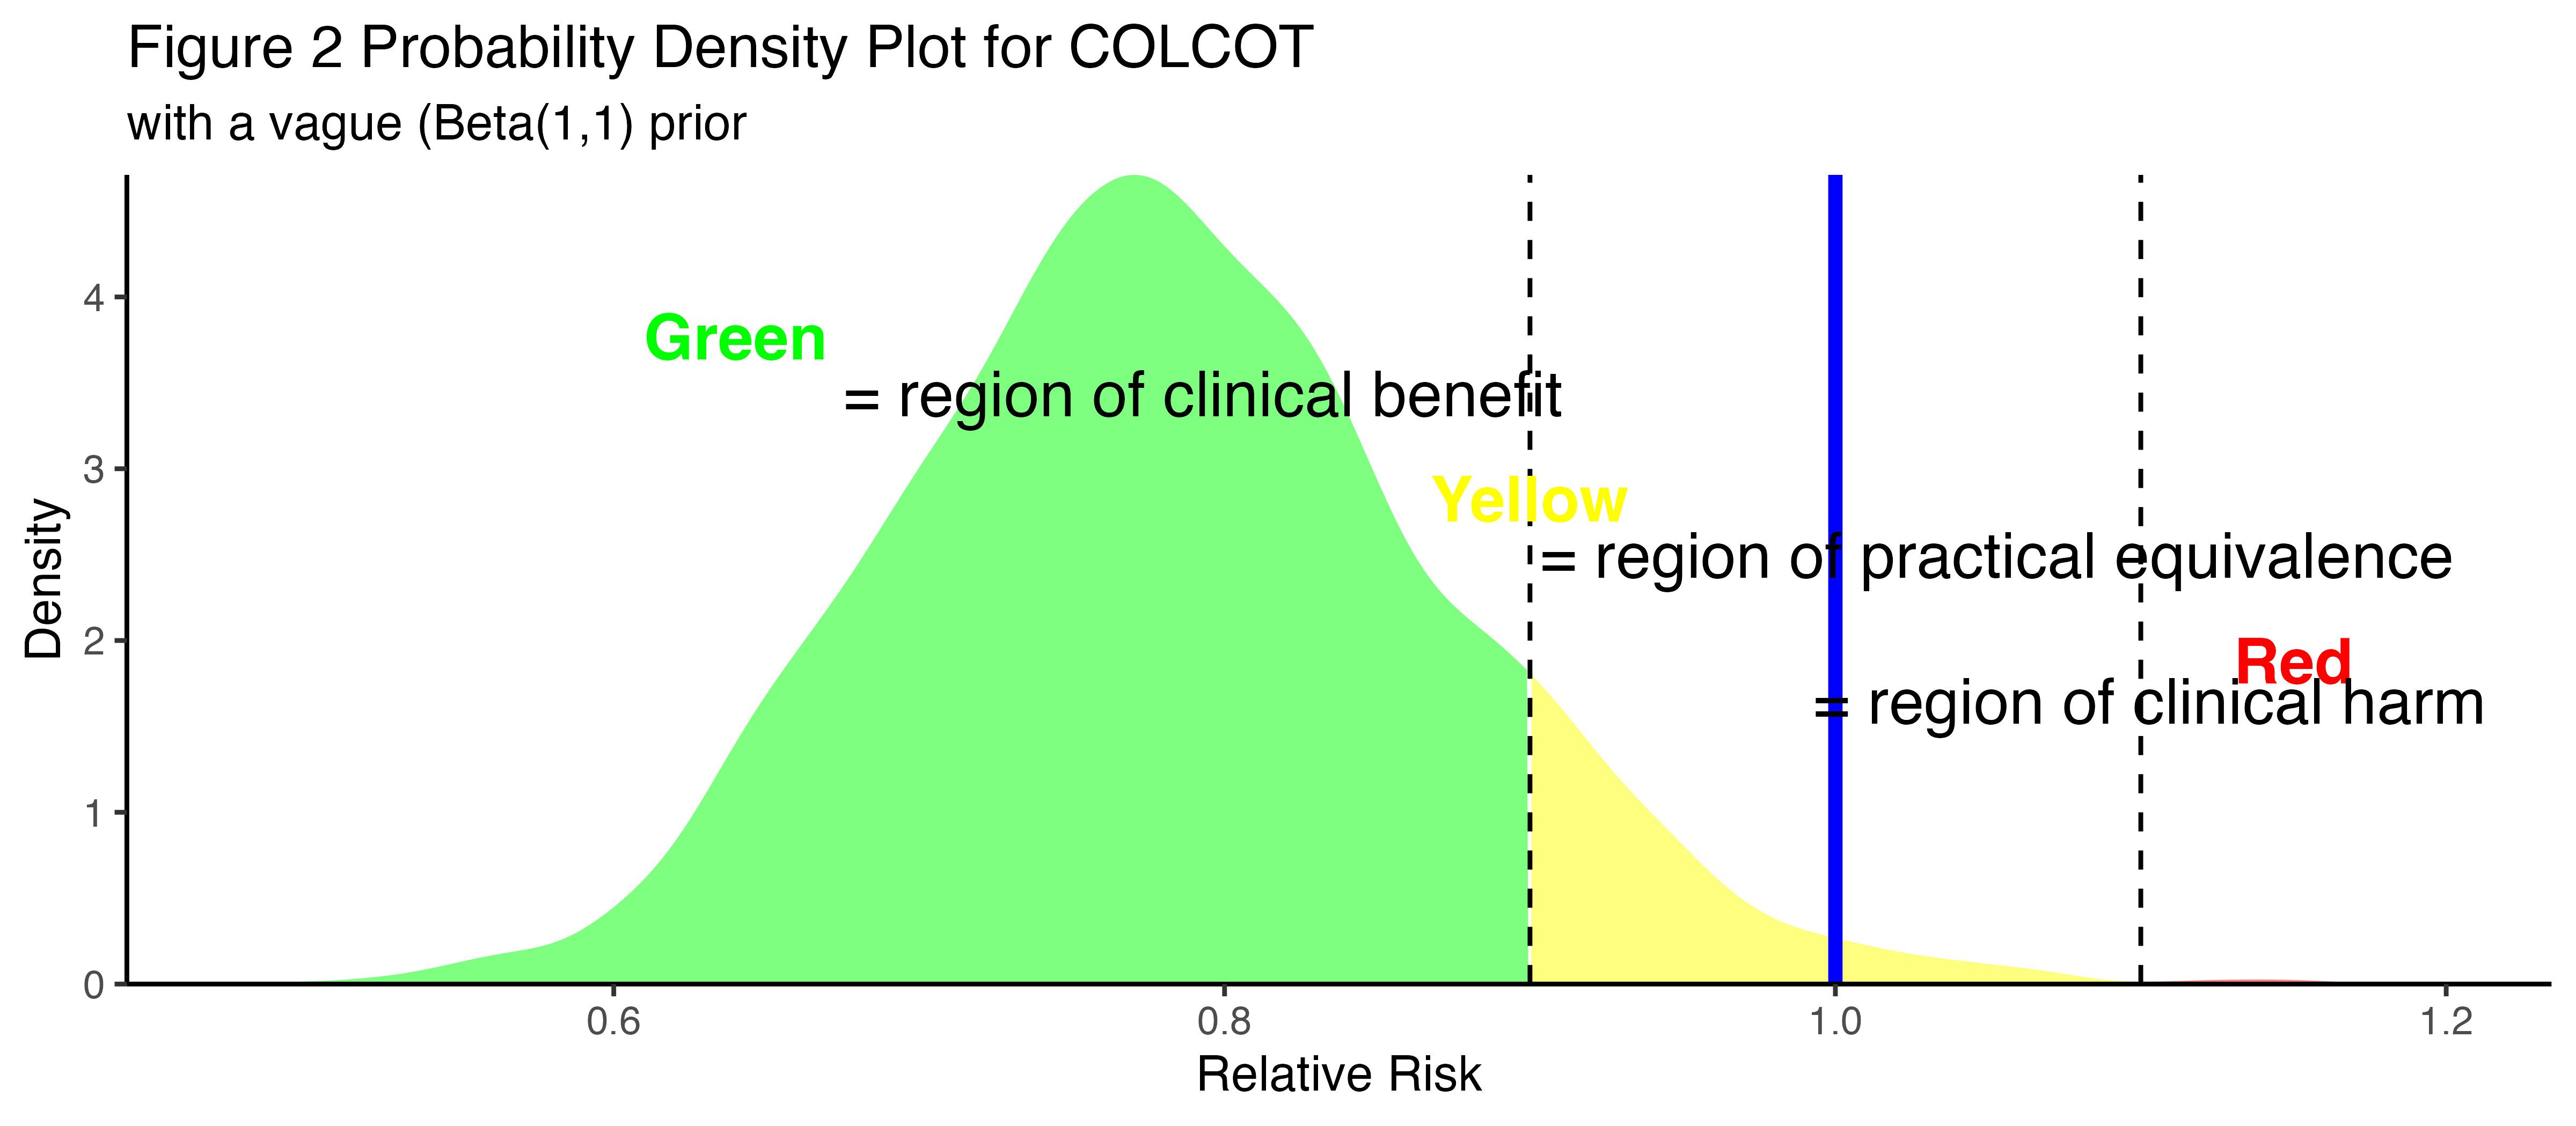
\includegraphics[keepaspectratio]{output/colcot_vague.png}}\\
\pandocbounded{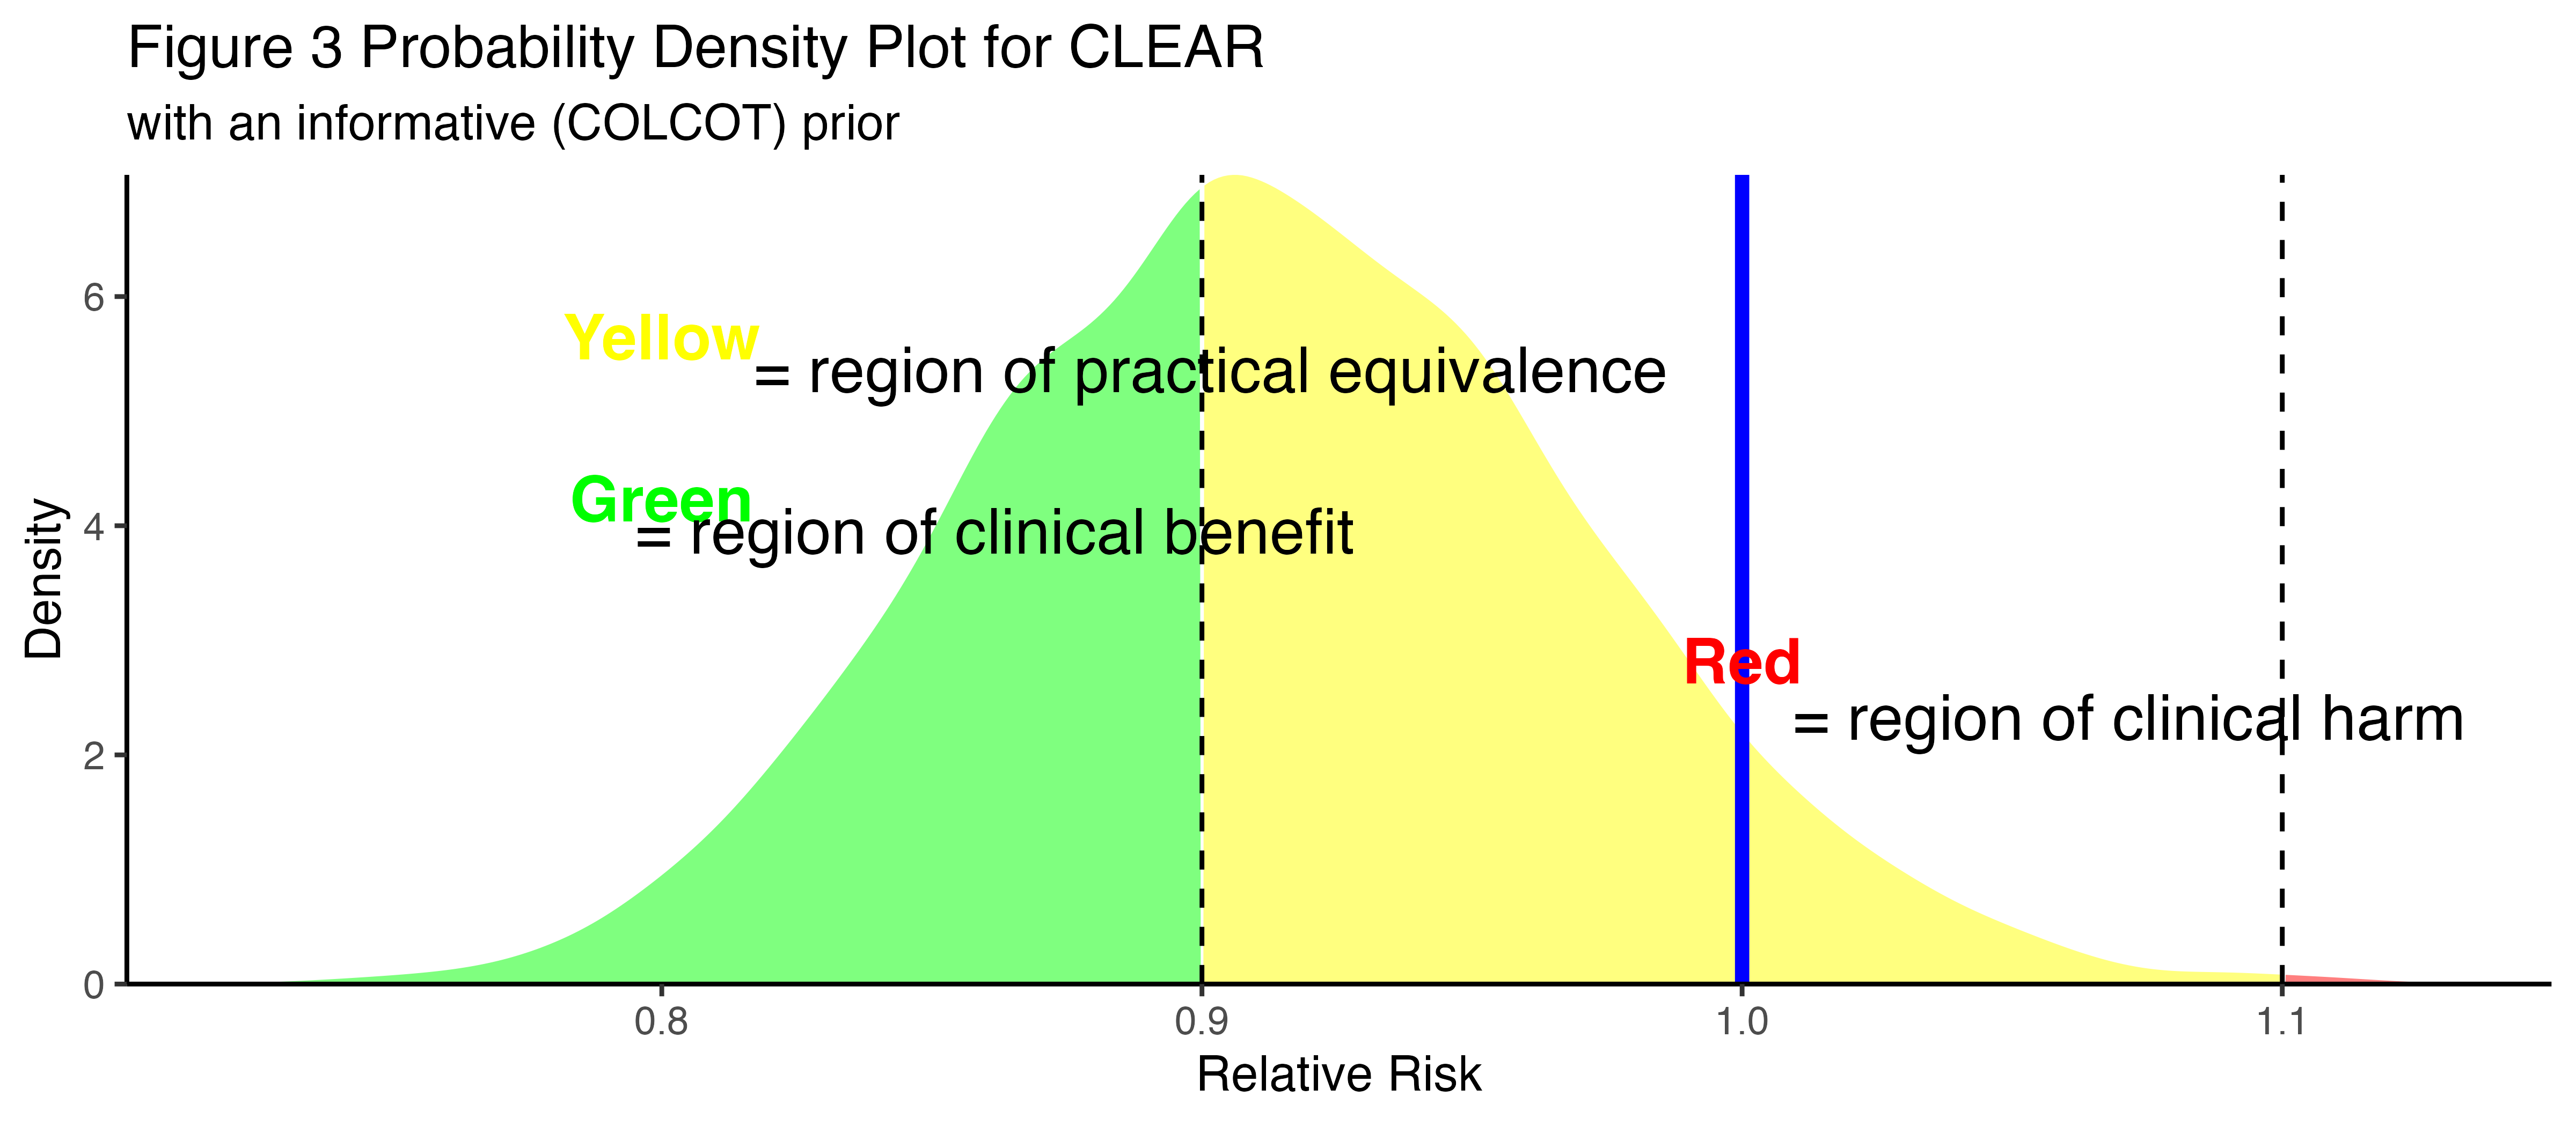
\includegraphics[keepaspectratio]{output/clear_colcot.png}}~
\pandocbounded{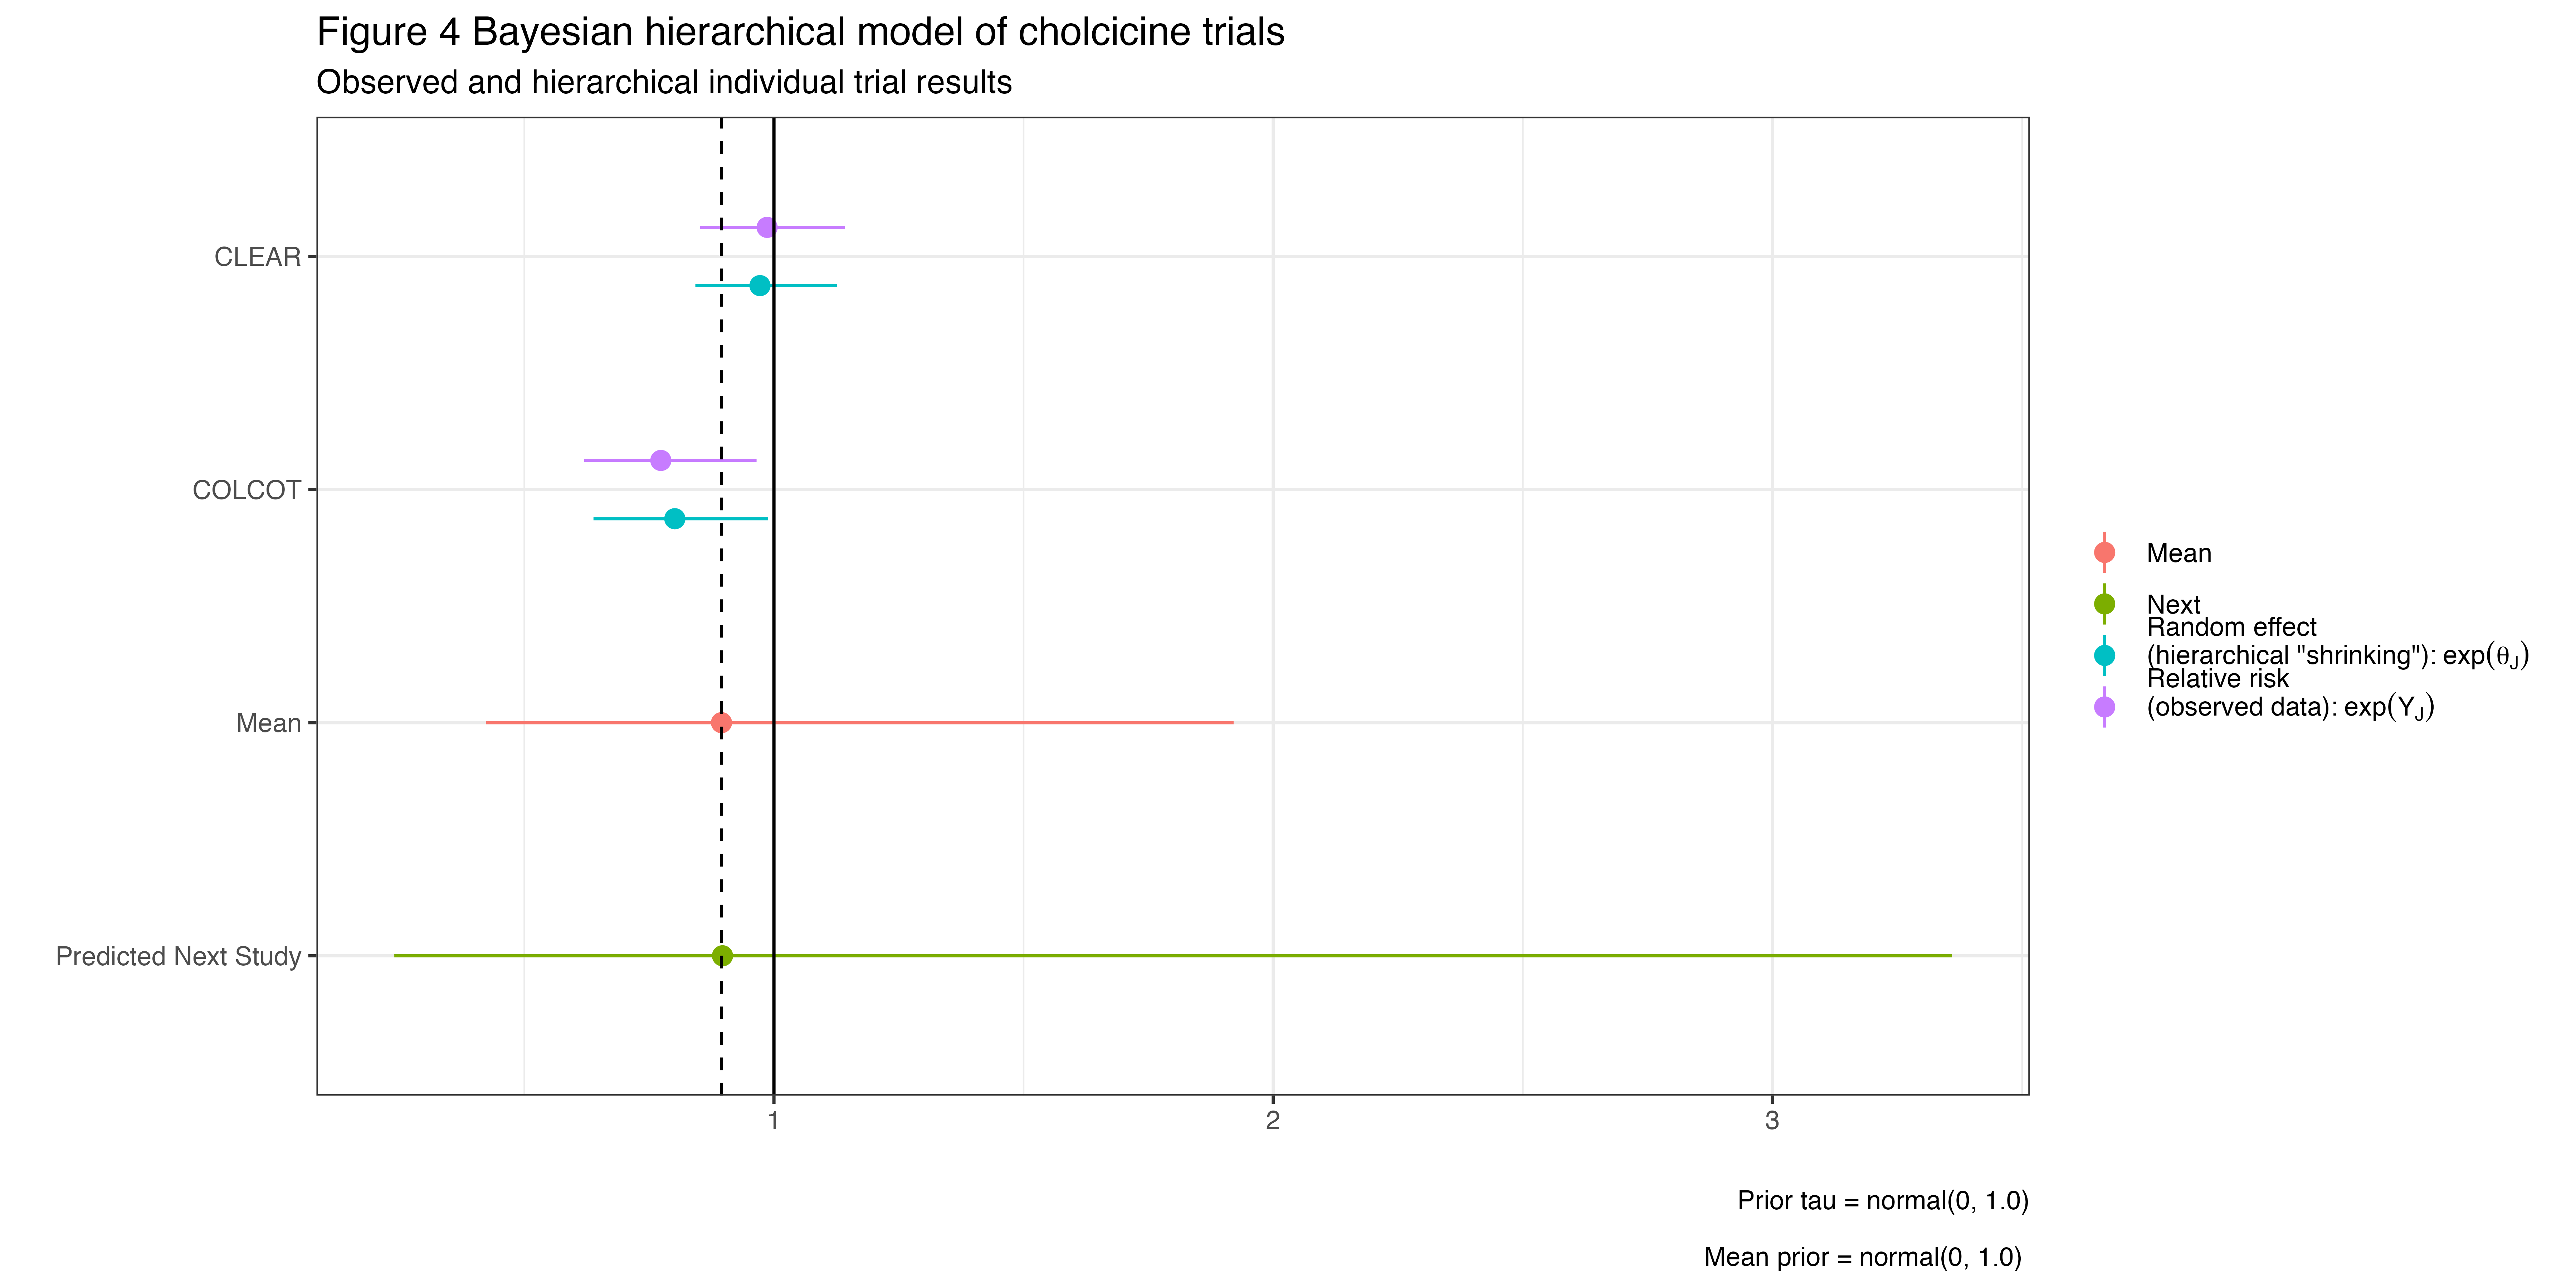
\includegraphics[keepaspectratio]{output/brms_hier.png}}\\

\subsection*{References}\label{references}
\addcontentsline{toc}{subsection}{References}

\phantomsection\label{refs}
\begin{CSLReferences}{0}{1}
\bibitem[\citeproctext]{ref-CLEAR}
\CSLLeftMargin{1. }%
\CSLRightInline{Jolly SS, d'Entremont MA, Lee SF, Mian R, Tyrwhitt J,
Kedev S, et al. Colchicine in acute myocardial infarction. New England
Journal of Medicine {[}Internet{]}. 0(0). Available from:
\url{https://www.nejm.org/doi/full/10.1056/NEJMoa2405922}}

\bibitem[\citeproctext]{ref-RN33}
\CSLLeftMargin{2. }%
\CSLRightInline{Tardif JC, Kouz S, Waters DD, Bertrand OF, Diaz R,
Maggioni AP, et al. Efficacy and safety of low-dose colchicine after
myocardial infarction. N Engl J Med. 2019;381(26):2497--505. }

\bibitem[\citeproctext]{ref-RN52}
\CSLLeftMargin{3. }%
\CSLRightInline{Kelly P, Lemmens R, Weimar C, Walsh C, Purroy F, Barber
M, et al. Long-term colchicine for the prevention of vascular recurrent
events in non-cardioembolic stroke (CONVINCE): A randomised controlled
trial. Lancet. 2024;404:125--33. }

\bibitem[\citeproctext]{ref-RN53}
\CSLLeftMargin{4. }%
\CSLRightInline{Li J, Meng X, Shi FD, Jing J, Gu HQ, Jin A, et al.
Colchicine in patients with acute ischaemic stroke or transient
ischaemic attack (CHANCE-3): Multicentre, double blind, randomised,
placebo controlled trial. BMJ. 2024;385:e079061. }

\bibitem[\citeproctext]{ref-RN7043}
\CSLLeftMargin{5. }%
\CSLRightInline{Lou N. Colchicine goes belly-up in a more definitive
heart attack trial {[}Internet{]}. 2024. Available from:
\url{https://www.medpagetoday.com/meetingcoverage/tct/112644?xid=nl_mpt_Cardiology_update_2024-11-01&mh=5ea0ef63b494fbd59d59b80f4d7177fa&zdee=gAAAAABm4utWmSHJnY-b0PoghpwIdJ2Z5bp7pHCJbHd4lnSWdd-TcQH64qhAqr5vStSuTwshVLoWZmIfruyxrtdHQaON6GGWin0MsBBlzSgmQd4CbqGcFWQ\%3D&utm_source=Sailthru&utm_medium=email&utm_campaign=Automated\%20Specialty\%20Update\%20Cardiology\%20BiWeekly\%20FRIDAY\%202024-11-01&utm_term=NL_Spec_Cardiology_Update_Active}}

\bibitem[\citeproctext]{ref-RN3836}
\CSLLeftMargin{6. }%
\CSLRightInline{Wasserstein RL, Lazar NA. The ASA's statement on
p-values: Context, process, and purpose. The American Statistician.
2016;70:2:129--33. }

\bibitem[\citeproctext]{ref-RN3826}
\CSLLeftMargin{7. }%
\CSLRightInline{Greenland S, Senn SJ, Rothman KJ, Carlin JB, Poole C,
Goodman SN, et al. Statistical tests, p values, confidence intervals,
and power: A guide to misinterpretations. European journal of
epidemiology. 2016;31(4):337--50. }

\bibitem[\citeproctext]{ref-RN5420}
\CSLLeftMargin{8. }%
\CSLRightInline{Wasserstein RL, Schirm AL, Lazar NA. Moving to a world
beyond {``p \textless{} 0.05.''} The American Statistician.
2019;73:1--19. }

\bibitem[\citeproctext]{ref-RN5721}
\CSLLeftMargin{9. }%
\CSLRightInline{Gelman A, Stern HS. The difference between
{``significant''} and {``not significant''} is not itself statistically
significant. 2006; }

\bibitem[\citeproctext]{ref-RN7045}
\CSLLeftMargin{10. }%
\CSLRightInline{Zwet E van, Wi!cek W, Gelman A. 2024. Available from:
\url{chrome-extension://efaidnbmnnnibpcajpcglclefindmkaj/https://stat.columbia.edu/~gelman/research/unpublished/Meta_analysis_with_a_single_trial.pdf}}

\end{CSLReferences}




\end{document}
